%-----------------------------------------------------------------------------------------------------------------------------------------------%
%	The MIT License (MIT)
%
%	Copyright (c) 2019 Jan Küster
%
%	Permission is hereby granted, free of charge, to any person obtaining a copy
%	of this software and associated documentation files (the "Software"), to deal
%	in the Software without restriction, including without limitation the rights
%	to use, copy, modify, merge, publish, distribute, sublicense, and/or sell
%	copies of the Software, and to permit persons to whom the Software is
%	furnished to do so, subject to the following conditions:
%
%	THE SOFTWARE IS PROVIDED "AS IS", WITHOUT WARRANTY OF ANY KIND, EXPRESS OR
%	IMPLIED, INCLUDING BUT NOT LIMITED TO THE WARRANTIES OF MERCHANTABILITY,
%	FITNESS FOR A PARTICULAR PURPOSE AND NONINFRINGEMENT. IN NO EVENT SHALL THE
%	AUTHORS OR COPYRIGHT HOLDERS BE LIABLE FOR ANY CLAIM, DAMAGES OR OTHER
%	LIABILITY, WHETHER IN AN ACTION OF CONTRACT, TORT OR OTHERWISE, ARISING FROM,
%	OUT OF OR IN CONNECTION WITH THE SOFTWARE OR THE USE OR OTHER DEALINGS IN
%	THE SOFTWARE.
%
%
%-----------------------------------------------------------------------------------------------------------------------------------------------%


%============================================================================%
%
%	DOCUMENT DEFINITION
%
%============================================================================%

%we use article class because we want to fully customize the page and don't use a cv template
\documentclass[10pt,A4]{article}


%----------------------------------------------------------------------------------------
%	ENCODING
%----------------------------------------------------------------------------------------

% we use utf8 since we want to build from any machine
\usepackage[utf8]{inputenc}

%----------------------------------------------------------------------------------------
%	LOGIC
%----------------------------------------------------------------------------------------

% provides \isempty test
\usepackage{xstring, xifthen}

%----------------------------------------------------------------------------------------
%	FONT BASICS
%----------------------------------------------------------------------------------------

% some tex-live fonts - choose your own

%\usepackage[defaultsans]{droidsans}
%\usepackage[default]{comfortaa}
%\usepackage{cmbright}
\usepackage[default]{raleway}
%\usepackage{fetamont}
%\usepackage[default]{gillius}
%\usepackage[light,math]{iwona}
%\usepackage[thin]{roboto}

% set font default
\renewcommand*\familydefault{\sfdefault}
\usepackage[T1]{fontenc}

% more font size definitions
\usepackage{moresize}

%----------------------------------------------------------------------------------------
%	FONT AWESOME ICONS
%----------------------------------------------------------------------------------------

% include the fontawesome icon set
\usepackage{fontawesome}

% use to vertically center content
% credits to: http://tex.stackexchange.com/questions/7219/how-to-vertically-center-two-images-next-to-each-other
\newcommand{\vcenteredinclude}[1]{\begingroup
\setbox0=\hbox{\includegraphics{#1}}%
\parbox{\wd0}{\box0}\endgroup}

% use to vertically center content
% credits to: http://tex.stackexchange.com/questions/7219/how-to-vertically-center-two-images-next-to-each-other
\newcommand*{\vcenteredhbox}[1]{\begingroup
\setbox0=\hbox{#1}\parbox{\wd0}{\box0}\endgroup}

% icon shortcut
\newcommand{\icon}[3] {
	\makebox(#2, #2){\textcolor{maincol}{\csname fa#1\endcsname}}
}

% icon with text shortcut
\newcommand{\icontext}[4]{
	\vcenteredhbox{\icon{#1}{#2}{#3}}  \hspace{2pt}  \parbox{0.9\mpwidth}{\textcolor{#4}{#3}}
}

% icon with website url
\newcommand{\iconhref}[5]{
    \vcenteredhbox{\icon{#1}{#2}{#5}}  \hspace{2pt} \href{#4}{\textcolor{#5}{#3}}
}

% icon with email link
\newcommand{\iconemail}[5]{
    \vcenteredhbox{\icon{#1}{#2}{#5}}  \hspace{2pt} \href{mailto:#4}{\textcolor{#5}{#3}}
}

\newcommand{\toto}[5]{
	\vcenteredhbox{\icon{star}}  \hspace{2pt} \href{mailto:#4}{\textcolor{#5}{#3}}
}

%----------------------------------------------------------------------------------------
%	PAGE LAYOUT  DEFINITIONS
%----------------------------------------------------------------------------------------

% page outer frames (debug-only)
% \usepackage{showframe}

% we use paracol to display breakable two columns
\usepackage{paracol}

% define page styles using geometry
\usepackage[a4paper]{geometry}

% remove all possible margins
\geometry{top=1cm, bottom=1cm, left=1cm, right=1cm}

\usepackage{fancyhdr}
\pagestyle{empty}

% space between header and content
% \setlength{\headheight}{0pt}

% indentation is zero
\setlength{\parindent}{0mm}

%----------------------------------------------------------------------------------------
%	TABLE /ARRAY DEFINITIONS
%----------------------------------------------------------------------------------------

% extended aligning of tabular cells
\usepackage{array}

% custom column right-align with fixed width
% use like p{size} but via x{size}
\newcolumntype{x}[1]{%
>{\raggedleft\hspace{0pt}}p{#1}}%


%----------------------------------------------------------------------------------------
%	GRAPHICS DEFINITIONS
%----------------------------------------------------------------------------------------

%for header image
\usepackage{graphicx}

% use this for floating figures
% \usepackage{wrapfig}
% \usepackage{float}
% \floatstyle{boxed}
% \restylefloat{figure}

%for drawing graphics
\usepackage{tikz}
\usetikzlibrary{shapes, backgrounds,mindmap, trees}

%----------------------------------------------------------------------------------------
%	Color DEFINITIONS
%----------------------------------------------------------------------------------------
\usepackage{transparent}
\usepackage{color}

% primary color
\definecolor{maincol}{RGB}{ 225, 0, 0 }

% accent color, secondary
% \definecolor{accentcol}{RGB}{ 250, 150, 10 }

% dark color
\definecolor{darkcol}{RGB}{ 70, 70, 70 }

% light color
\definecolor{lightcol}{RGB}{245,245,245}


% Package for links, must be the last package used
\usepackage[hidelinks]{hyperref}

% returns minipage width minus two times \fboxsep
% to keep padding included in width calculations
% can also be used for other boxes / environments
\newcommand{\mpwidth}{\linewidth-\fboxsep-\fboxsep}



%============================================================================%
%
%	CV COMMANDS
%
%============================================================================%

%----------------------------------------------------------------------------------------
%	 CV LIST
%----------------------------------------------------------------------------------------

% renders a standard latex list but abstracts away the environment definition (begin/end)
\newcommand{\cvlist}[1] {
	\begin{itemize}{#1}\end{itemize}
}

%----------------------------------------------------------------------------------------
%	 CV TEXT
%----------------------------------------------------------------------------------------

% base class to wrap any text based stuff here. Renders like a paragraph.
% Allows complex commands to be passed, too.
% param 1: *any
\newcommand{\cvtext}[1] {
	\begin{tabular*}{1\mpwidth}{p{0.98\mpwidth}}
		\parbox{1\mpwidth}{#1}
	\end{tabular*}
}

%----------------------------------------------------------------------------------------
%	CV SECTION
%----------------------------------------------------------------------------------------

% Renders a a CV section headline with a nice underline in main color.
% param 1: section title
\newcommand{\cvsection}[1] {
	\vspace{14pt}
	\cvtext{
		\textbf{\LARGE{\textcolor{darkcol}{\uppercase{#1}}}}\\[-4pt]
		\textcolor{maincol}{ \rule{0.1\textwidth}{2pt} } \\
	}
}

%----------------------------------------------------------------------------------------
%	META SKILL
%----------------------------------------------------------------------------------------

% Renders a progress-bar to indicate a certain skill in percent.
% param 1: name of the skill / tech / etc.
% param 2: level (for example in years)
% param 3: percent, values range from 0 to 1
\newcommand{\cvskill}[3] {
	\begin{tabular*}{1\mpwidth}{p{0.72\mpwidth}  r}
 		\textcolor{black}{\textbf{#1}} & \textcolor{maincol}{#2}\\
	\end{tabular*}%

	\hspace{4pt}
	\begin{tikzpicture}[scale=1,rounded corners=2pt,very thin]
		\fill [lightcol] (0,0) rectangle (1\mpwidth, 0.15);
		\fill [maincol] (0,0) rectangle (#3\mpwidth, 0.15);
  	\end{tikzpicture}%
}


%----------------------------------------------------------------------------------------
%	 CV EVENT
%----------------------------------------------------------------------------------------

% Renders a table and a paragraph (cvtext) wrapped in a parbox (to ensure minimum content
% is glued together when a pagebreak appears).
% Additional Information can be passed in text or list form (or other environments).
% the work you did
% param 1: time-frame i.e. Sep 14 - Jan 15 etc.
% param 2:	 event name (job position etc.)
% param 3: Customer, Employer, Industry
% param 4: Short description
% param 5: work done (optional)
% param 6: technologies include (optional)
% param 7: achievements (optional)
\newcommand{\cvevent}[7] {

	% we wrap this part in a parbox, so title and description are not separated on a pagebreak
	% if you need more control on page breaks, remove the parbox
	\parbox{\mpwidth}{
		\begin{tabular*}{1\mpwidth}{p{0.72\mpwidth}  r}
	 		\textcolor{black}{\textbf{#2}} & \colorbox{maincol}{\makebox[0.30\mpwidth]{\textcolor{white}{#1}}} \\
			\textcolor{maincol}{\textbf{#3}} & \\
		\end{tabular*}\\[8pt]

		\ifthenelse{\isempty{#4}}{}{
			\cvtext{#4}\\
		}
	}

	\ifthenelse{\isempty{#5}}{}{
		\vspace{9pt}
		{#5}
	}

	\ifthenelse{\isempty{#6}}{}{
		\vspace{9pt}
		\cvtext{\textbf{Technos:}}\\
		{#6}
	}

	\ifthenelse{\isempty{#7}}{}{
		\vspace{9pt}
		\cvtext{\textbf{Réussites:}}\\
		{#7}
	}
	\vspace{14pt}
}

%----------------------------------------------------------------------------------------
%	 CV META EVENT
%----------------------------------------------------------------------------------------

% Renders a CV event on the sidebar
% param 1: title
% param 2: subtitle (optional)
% param 3: customer, employer, etc,. (optional)
% param 4: info text (optional)
\newcommand{\cvmetaevent}[4] {
	\textcolor{maincol} {\cvtext{\textbf{\begin{flushleft}#1\end{flushleft}}}}

	\ifthenelse{\isempty{#2}}{}{
	\textcolor{darkcol} {\cvtext{\textbf{#2}} }
	}

	\ifthenelse{\isempty{#3}}{}{
		\cvtext{{ \textcolor{darkcol} {#3} }}\\
	}

	\cvtext{#4}\\[14pt]
}

%---------------------------------------------------------------------------------------
%	QR CODE
%----------------------------------------------------------------------------------------

% Renders a qrcode image (centered, relative to the parentwidth)
% param 1: percent width, from 0 to 1
\newcommand{\cvqrcode}[1] {
	\begin{center}
		
\includegraphics[width={#1}\mpwidth]{qrcode}
	\end{center}
}


%============================================================================%
%
%
%
%	DOCUMENT CONTENT
%
%
%
%============================================================================%
\begin{document}
\columnratio{0.31}
\setlength{\columnsep}{2.2em}
\setlength{\columnseprule}{4pt}
\colseprulecolor{lightcol}
\begin{paracol}{2}
\begin{leftcolumn}
%---------------------------------------------------------------------------------------
%	META IMAGE
%----------------------------------------------------------------------------------------
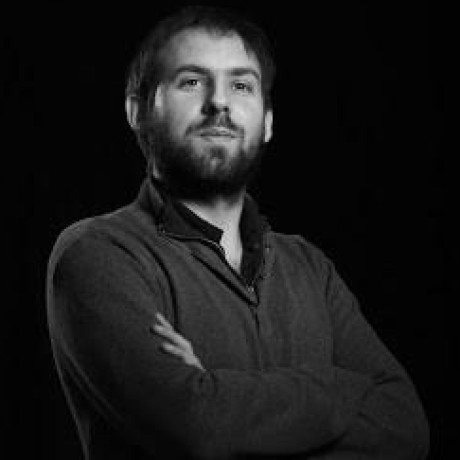
\includegraphics[width=\linewidth]{gwa.jpg}	%trimming relative to image size

%---------------------------------------------------------------------------------------
%	META SKILLS
%----------------------------------------------------------------------------------------
\cvsection{SKILLS}

\cvskill{Java/Spring} {10+ ans} {1} \\[-2pt]

\cvskill{TDD} {9+ ans} {1} \\[-2pt]

\cvskill{Linux} {15+ ans} {0.9} \\[-2pt]

\cvskill{React} {7+ ans} {0.9} \\[-2pt]

\cvskill{Typescript} {7+ ans} {0.8} \\[-2pt]

\cvskill{Docker} {7+ ans} {0.8} \\[-2pt]

\cvskill{Kubernetes} {7+ ans} {0.6} \\[-2pt]

\cvskill{Kotlin} {3+ ans} {0.7} \\[-2pt]



\vfill\null
\cvsection{CONTACT}

\icontext{MapMarker}{12}{CITY}{black}\\[6pt]
\icontext{MobilePhone}{12}{PHONE}{black}\\[6pt]
\iconemail{Envelope}{12}{mail}{mail@mail.com}{black}\\[6pt]

\vfill\null
\cvqrcode{0.7}

%---------------------------------------------------------------------------------------
%	EDUCATION
%----------------------------------------------------------------------------------------
\newpage
\cvsection{EDUCATION}

\cvmetaevent
{2005 - 2010}
{Igénieur développement}
{EPITA}
{BAC +5}

%---------------------------------------------------------------------------------------
%	PUBLICATIONS
%----------------------------------------------------------------------------------------
\cvsection{Publications}

\icontext{Book}{12}{Mastering Spring MVC 4\\Packt}{black}\\[6pt]
\icontext{Firefox}{12}{\href{https://geowarin.com}{geowarin.com}}{black}\\[6pt]

%---------------------------------------------------------------------------------------
%	LANGUES
%----------------------------------------------------------------------------------------
\cvsection{Langues}

\cvskill{Français} {Natal} {1} \\[-2pt]

\cvskill{Anglais} {Bilingue} {0.9} \\[-2pt]

\cvskill{Italien} {Notions} {0.4} \\[-2pt]

\vfill\null

%---------------------------------------------------------------------------------------
%	OPEN-SOURCE
%----------------------------------------------------------------------------------------
\newpage
\cvsection{Open-source}

\cvmetaevent
{\href{https://github.com/geowarin/friendly-errors-webpack-plugin}{friendly-errors-webpack-plugin}\\[6pt]}
{}
{\icon{Star}{12}{} 748}
{
Recognizes certain classes of webpack errors and cleans, aggregates and prioritizes
them to provide a better Developer Experience.
}

\cvmetaevent
{\href{https://github.com/geowarin/boot-react}{boot-react}\\[6pt]}
{}
{\icon{Star}{12}{} 601}
{
A starter application with spring boot and react
}

\cvmetaevent
{\href{https://github.com/geowarin/electron-hot-loader}{electron-hot-loader}\\[6pt]}
{}
{\icon{Star}{12}{} 194}
{
	A starter application with spring boot and react
}

\cvmetaevent
{}
{Et plus de 170 autres projets open-source !}
{}

\vfill

\end{leftcolumn}
\begin{rightcolumn}
%---------------------------------------------------------------------------------------
%	TITLE  HEADER
%----------------------------------------------------------------------------------------
\fcolorbox{white}{darkcol}{\begin{minipage}[c][3.5cm][c]{1\mpwidth}
	\begin {center}
		\HUGE{ \textbf{ \textcolor{white}{ \uppercase{ GEOFFROY WARIN } } } } \\[-24pt]
		\textcolor{white}{ \rule{0.1\textwidth}{1.25pt} } \\[4pt]
		\large{ \textcolor{white} {Développeur fullstack} }
	\end {center}
\end{minipage}} \\[14pt]
\vspace{-12pt}

%---------------------------------------------------------------------------------------
%	PROFILE
%----------------------------------------------------------------------------------------
\vfill\null
\cvsection{PROFIL}

\cvtext{
Je suis à l’aise avec les langages JVM (Java, Kotlin), le developpement
front (React, Typescript), les bases de données et les technologies cloud (docker, kubernetes).\\
}

\cvtext{J'adore coder mais également:}

{\cvlist{
	\item Le recrutement
	\item La facilitation de réunions (spring planning, rétrospectives, sessions de design)
	\item Donner des formations (2 ans en tant que formateur)
	\item Ecrire (j'ai rédigé un livre sur Spring MVC publié par Packt)
	\item Le pair programming et le TDD
}}


%---------------------------------------------------------------------------------------
%	WORK EXPERIENCE
%----------------------------------------------------------------------------------------
\vfill\null
\cvsection{Expériences}

\cvevent
{Depuis Fév 2021}
{Senior FullStack developer}
{Société Générale}
{Arrivé chez SG Markets pour travailler sur FX, une application mature et nécessitant une
réelle expertise technique, on m'a rapidement fait assez confiance pour la mise en place de deux nouveaux
projets: \\
FX TCA (Transaction Cost Analysis), mis en production en juin 2022, et TREE (Target Risk Engine for Equity) sur lequel je travaille actuellement.}
{\cvlist{
	\item Expertise technique
	\item Recrutement
}}
{\cvlist {
	\item React/Typescript
	\item Jenkins/ArgoCD/Azure
}}
{\cvlist{
	\item Chantier de migration des tests E2E FX
	\item Conception et mise en prod de FX TCA (Live charts)
	\item Mise en place de l'architecture TREE
}}

\vfill\null
\cvevent
{Mai 2019 - Mai 2020}
{BiSam/FacSet}
{Senior Software Engineering Manager}
{En 2019, j'ai managé une équipe de 5 personnes en charge de l'application Portfolio Vault De FactSet.
\\\\Il s'agit d'une application SaaS déployée avec Kubernetes sur AWS exposant une API GraphQL.
}
	{\cvlist{
		\item Recrutement
		\item Mentorat
		\item Organisation du travail
	}}
	{\cvlist {
		\item Docker, Kubernetes, AWS
		\item GraphQL
	}}
	{\cvlist{
		\item Réappropriation par l'équipe de la chaine de production de l'application
		\item Accompagnement de l'équipe dans le changement de stratégie de l'entreprise suite au rachat par FactSet
	}}

\vfill\null
\cvevent
{Mai 2018 - Mai 2019}
{BiSam/FacSet}
{Senior Software Engineer}
{J'ai aidé les équipe de BiSam/FacSet a créer une nouvelle application web à partir de l'application legacy Swing.
\\\\La nouvelle stack était constituée de Vaadin et de Polymer et a posé les bases de la nouvelle application
GIPS de FactSet en terme d'expérience utilisateur (UX).
}
{\cvlist{
	\item Migrations de code automatiques nécessitant une bonne connaissance de Java et de Javascript
	\item Participation à l'élaboration de la nouvelle UX avec les product owners
}}
{\cvlist {
	\item Vaadin, Polymer
}}
{\cvlist{
	\item Refactorings importants pour la migration ainsi que la perennité de l'application legacy
	\item Conception d'un moulinette capable de migrer des écrans Swing en Vaadin
	\item Formation des équipes aux paradigmes du Web
}}

\vfill\null
\cvevent
{Jan 2017 - Fév 2018}
{Mon Gérant Privé}
{CTO}
{En tant quie CTO d'une fintech, mon rôle a été de créer les foncation d'une application de gestion de
portefeuilles à la pointe de la technologie.}
{\cvlist{
	\item Sélection des Technos
	\item Rectrutement
	\item Participation aux avant-ventes
}}
{\cvlist {
	\item React + Typescript
	\item Spring Boot + JooQ + Kotlin
}}
{\cvlist{
	\item Equipe sélectionnée pour intégrer l'incubateur de la Société Générale
}}

\vfill\null
\cvevent
{Mai 2016 - Juin 2016}
{MNT - Mutuelle Nationale Territoriale}
{Lead dev React- Freelance}
{A la MNT, j'ai conçu la première application React du groupe.\\\\
Le projet était d'importance critique car il devait permettre aux employés d'accéder aux documents
de l'entreprise pendant le grand chantier de numérisation des dossiers.}
{\cvlist{
	\item Conception d'un framework pour les prochaines applications React du groupe
	\item Mise en place de l'intégration continue
	\item Participation à la mise en place de Docker
}}
{\cvlist {
	\item React
	\item GoCD
}}
{\cvlist{
	\item Mentoring du développeut backend
	\item Conception de l'architecture en collaboration avec les différents services du groupe
}}

\vfill\null
\cvevent
{Avr 2013 - Mai 2016}
{BiSam}
{Javascript / Cloud developper}
{En mai 2015, j’ai intégré BiSam en tant qu’employé et j’ai continué à
développer leur application SaaS à destination des gestionnaires de
fonds, BiSam-GO.\\
En tant que tech lead, mon rôle était d’épauler l’équipe ainsi que de
travailler en forte collaboration avec les architectes pour déployer
l’application dans un cluster Kubernetes.\\\\
En Octobre, j’ai intégré l’équipe architecture où ma mission était de
maintenir l’application qui permet à l’équipe de production de gérer les
clusters Kubernetes déployés sur Rackspace.\\
L’application est écrite en React, Groovy et Spring boot et utilise les
websockets pour afficher en direct l’état du cluster.}
{\cvlist{
	\item Recrutement
	\item Conception du pipeline Jenkins de déploiement continu (groovy)
	\item Pair programming à temps plein
	\item TTD, Scrum, Lean
}}
{\cvlist {
	\item React/Groovy/Spring Boot/Chef
	\item BackboneJS/Jersey
}}
{\cvlist{
	\item Avoir travaillé dans toutes les équipes de développement de l’entreprise (4)
	\item Avoir maîtrisé l’art du TDD grâce à mon mentor et des projets après les horaires de bureau
	\item En parallèle, écriture d’un livre sur Spring MVC
}}

\vfill\null
\cvevent
{2013 - 2014}
{Xebia}
{Consultant}
{Durant mes 2 ans en tant que consultant chez Xebia, je travaillaise chez
BiSam pour les aider à développer leur application SaaS, BiSam-GO.\\\\
Xebia est une société de service très active avec un gros accent
sur la qualité de code et la satisfaction client.}
{\cvlist{
	\item Tribu Software Craftmanship
	\item Xebia essentials
}}
{}
{}

\vfill\null
\cvevent
{Avr 2010 - Déc 2012}
{Middleware Factory}
{Expert technique}
{Pendant mes 2 ans en tant que consultant chez Middleware Factory, j’ai
aidé mes clients à développer des applications web et à mettre en place
des environnement d’intégration continue.
Je travaillais avec eux pour accroître la qualité des logiciels au moyen
d’audit de code, en leur proposant des migrations vers de nouvelles technologies et en prodiguant des conseils d’architecture.
Ces missions étaient principalement dans des environnements JEE avec
un gros accent sur JSF où j’ai construit une expertise forte.}
{\cvlist{
	\item Bougues Telecom - Lead Developper - Mai 2010 - Mai 2011
	\item ING Direct - Technical Expert/ JSF - Juin 2011 - Décembre 2012
	\item STIME/ Intermarché - Expert/ Architect - Janvier 2012 - Décembre 2012
}}
{\cvlist {
	\item JSF, Maven
}}
{\cvlist{
	\item Référent technique dans les différentes équipes
	\item En parallèle, formateur indépendant
}}

% hotfixes to create fake-space to ensure the whole height is used
\mbox{}
\vfill
\mbox{}
\vfill
\mbox{}
\vfill
\mbox{}
\end{rightcolumn}
\end{paracol}
\end{document}

